\section{Experimental Design}
\label{sec:design}

The design compares four defence layers against nine log types on a field that
deliberately violates every assumption of the twin: if the field were generated
by the twin itself, a $0/60$ false-accusation rate would measure only
self-consistency (Supplementary~S10.4), so here the field is generated by a
separate process that
differs from the twin along seven axes, each with a published source (every
value in Supplementary Table~S5; axis-by-axis list and per-event recording
semantics in S20.1). Weather is hourly ERA5~\cite{hersbach2020} (Open-Meteo archive) for Can Tho,
Soc Trang and Ca Mau over 2024 (water-scarce) and 2025 (water-surplus), window
1 March to 29 May ($2\,160$\,h), the dry season in which AWD is
practised~\cite{tuong2003}. Layer~1 is the point-model detector (default profile, absolute
threshold $\tau_0=5$\,mm); Layer~2 the robust detector of \eqref{eq:robust}
with the proportional threshold of \eqref{eq:tau}, on both a reduced
$\Theta$ ($24$ replays per log, $10$ seeds) and the full one ($150$ replays,
cross-check); Layer~3 the device anchor of \eqref{eq:anchor}; Layer~4 physics
alone, for reference. Of the nine log types, two are honest (paper and field conditions), three are naive
forgeries and four adversarial, built by
an optimiser rather than a fixed recipe (full list in S16); all attack
statistics are conditioned on a \texttt{changed} flag, because an adversary
that finds no improving move returns the original log, and comparisons use the
baseline of the variant itself (two harness defects, S10.2). For each layer we
report the escape rate (forged logs neither physical tier flags) and the
false-accusation rate on honest logs; for credit impact, $n_{\mathrm{dry}}$ of
\eqref{eq:ndry} against the honest field baseline, paired. Volume appears only
as a diagnostic (S10.3).

\section{Results}
\label{sec:results}

\subsection{The point-model detector is unsafe, not merely optimistic}

Table~\ref{tab:falseacc} gives the central negative result: the point-model
detector accuses nobody on paper-condition logs, reproducing the $0/60$ of the
self-consistency protocol,
but accuses $26.7\%$ of honest farmers on field-condition logs. The cause is
\eqref{eq:gap} with an absolute threshold --- forgetting, rounding or a
day-late entry all produce $G>5$\,mm without wrongdoing; the measured gap on
honest field-condition logs reached $65$\,mm. The proportional threshold of
\eqref{eq:tau} cuts this to $5.0\%$, the device anchor to $0/60$.

\subsection{Physics cannot see the attack that pays}
\label{sec:results-attack}

\begin{figure}[!t]
\centering
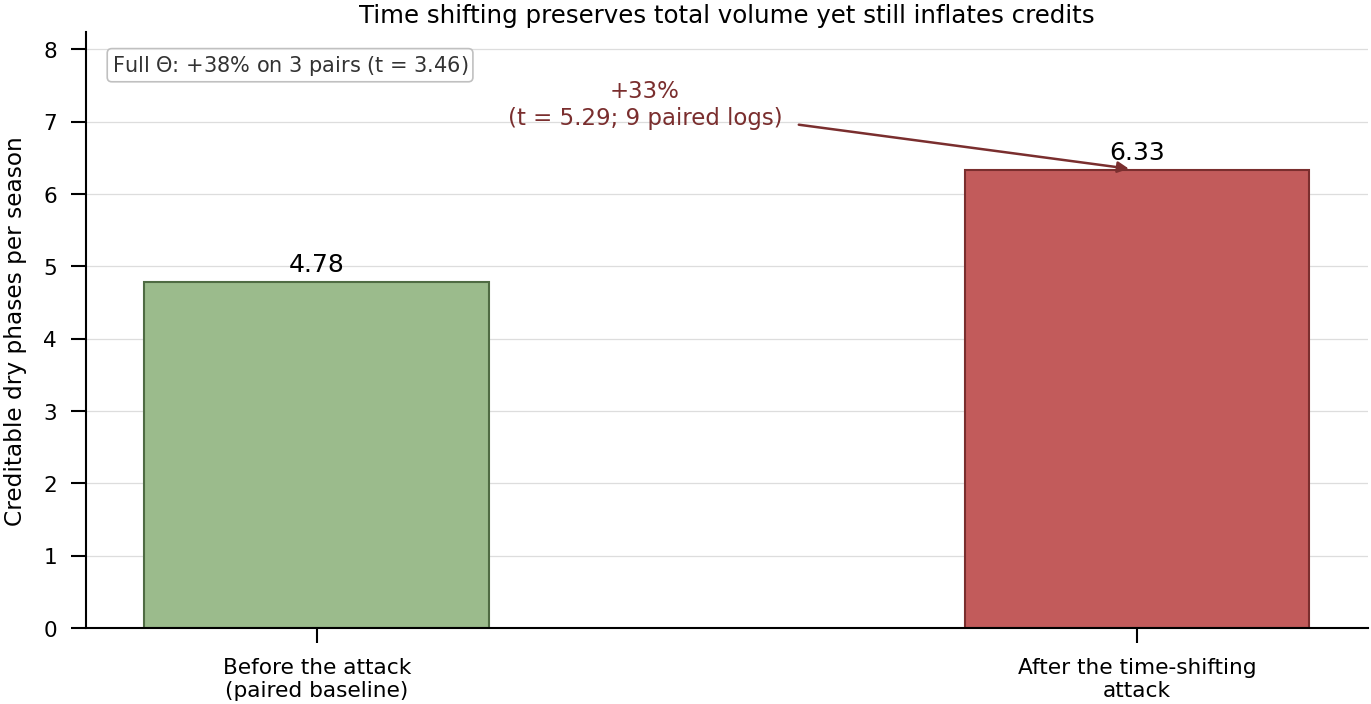
\includegraphics[height=6.9cm]{figures_vi/fig3_timeshift_en.png}
\caption{The time-shifting attack on the paired subset: creditable dry phases before and after moving the command timestamps, with the total volume and every individual depth preserved. The gain under the full uncertainty set is noted at the lower right.}\label{fig:timeshift}
\end{figure}

Fig.~\ref{fig:timeshift} plots that paired comparison. Table~\ref{tab:credit} is the second negative result, and the one that matters
economically. Every inflation figure is a \emph{paired} comparison against the
honest log of the same trajectory, restricted to attacks that actually changed
the record; the unpaired alternative overstates the gain roughly twofold (S15).
Time-shifting raises creditable dry phases from $4.78$ to $6.33$ per season,
$+33\%$ over nine altered logs ($t=5.29$); under the full uncertainty set,
$+38\%$ over three ($t=3.46$, $p=0.074$ --- directionally consistent but not
significant at $0.05$ with this sample); the rational adversary reaches $+35\%$
and $+40\%$ ($p=0.007$ and $p=0.30$). Consolidation gains almost nothing once paired ($+1\%$, $+2\%$),
and the two crude forgeries \emph{reduce} creditable phases ($-1\%$,
$-17\%$): only the volume-preserving permutation of timestamps is profitable,
as Proposition~\ref{prop:coincide} predicts. The escape rates in Table~\ref{tab:defence} are the heart of the result:
time-shifting escapes the robust physics layer in $8$ of $9$ altered logs, the
rational adversary in $6$ of $6$. The point model catches more ($4$ of $9$),
but it is precisely the detector that accuses $26.7\%$ of honest farmers; the
robust tier cuts that to $5.0\%$ and hands most of the detection back ($1$ of
$9$) --- \emph{no physical configuration escapes that trade-off}, because
both tiers are functions of the replayed trajectory. The infiltration filter $V_5$ fires $648$ times, but exclusively on the crude
depth-inflation forgery: useful, and orthogonal to the threat that pays.

\begin{figure}[!t]
\centering
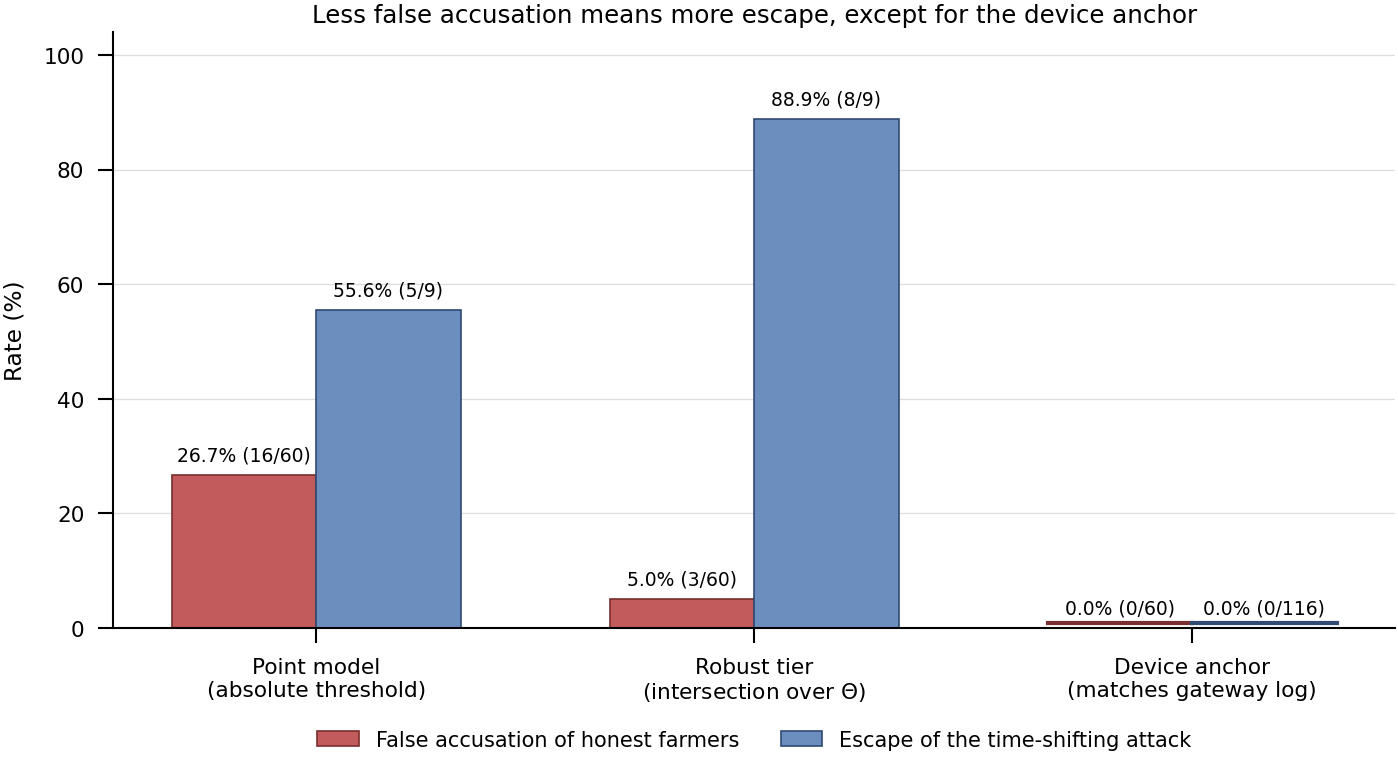
\includegraphics[height=6.9cm]{figures_vi/fig2_tradeoff_en.png}
\caption{Trade-off between the two error types across the three defence tiers. Lowering the false-accusation rate raises the escape rate of the time-shifting attack; only the device anchor reaches zero on both.}\label{fig:tradeoff}
\end{figure}

\subsection{The anchor closes every class, and the cost of robustness}

Fig.~\ref{fig:tradeoff} summarises the trade-off measured in the two preceding subsections. Table~\ref{tab:defence} also gives the constructive half. All $281$ logs were
audited under the reduced uncertainty set, of which $85$ were re-audited under
the full one (Supplementary~S17.2). Of the $281$ logs, $116$ were genuinely altered, and the device anchor caught $116/116$
while accusing none of $60$ honest field-condition logs ($37/37$ and $0/18$
under the full $\Theta$). Naive forgeries are caught by every layer; the
distinction lies in the adversarial rows, where only the anchor holds.
Robustness is not free: on the nine
omission-fraud logs actually altered the point model catches $9/9$, the robust
rule $4/9$ ($4/4$ vs $2/4$ full $\Theta$) --- a loss of detection power, not
a Pareto improvement, though the correct side of the trade. Every conclusion
holds under both the reduced $\Theta$ ($24$ replays, $281$ logs, $10$ seeds)
and the full one ($150$ replays, $85$ logs, $3$ seeds): false accusation
$0/60$ and $0/18$, anchor completeness $116/116$ and $37/37$, time-shift
escape $8/9$ and $3/3$, paired inflation $+33\%$ and $+38\%$
(Supplementary~S17).
